\section{Vista Lógica}
En la figura \ref{fig:Diagrama de Clases - Vista Logica} se muestra un diagrama de clases que conforman la estructura de la base de datos para poder manipularla a través del sistema. Consta de 4 clases: Mecanico, Vehiculo, Refaccion, Solicitud. La clase Mecanico hereda de la clase Vehiculo que a su vez hereda de Refaccion y de Solicitud, esto para poder tener una relación entre todos los datos. En otras palabras, un Mecánico puede tener uno o varios Vehículos en el taller y estos mismos pueden necesitar una Refacción, estas a su vez pueden ser obtenidas mediante una Solicitud. 
Los atributos de cada clase son los siguientes: 
\begin{itemize}
	\item \textbf{Mecanico:}El nombre de usuario y contraseña.
	\item \textbf{Vehiculo:}El numero de inventario, la descripción del vehiculo (puede ser el modelo o señas particulares), la fecha de entrada y de salida además del procedimiento que se debe de realizar.
	\item \textbf{Refaccion:}El numero de inventario y la descripción de la refacción (para que vehículo funciona o señas particulares de la pieza).
	\item \textbf{Solicitud:}Identificador de la solicitud y fecha de la misma.
\end{itemize}
\begin{figure}[!h]
	\centering
	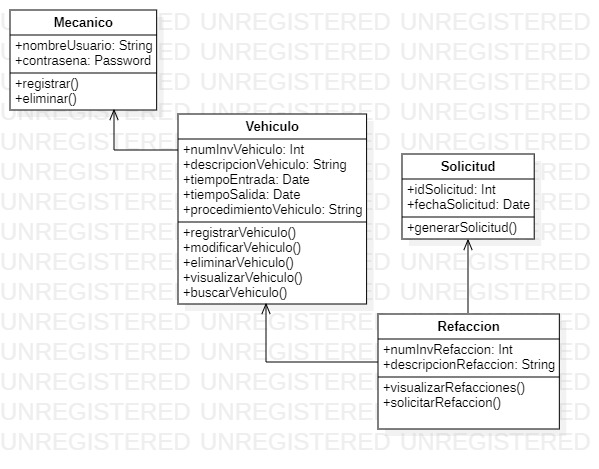
\includegraphics[width=0.8\textwidth]{./diseno/vlogica/imagenes/vistaLogica}
	\caption{Diagrama de Clases - Vista Lógica}
	\label{fig:Diagrama de Clases - Vista Logica}
\end{figure}
\clearpage